\documentclass[tikz,border=5pt]{standalone}
\usepackage{pgfplots}
\pgfplotsset{compat=1.18}

\definecolor{corba}{HTML}{365FB3}
\definecolor{punt}{HTML}{B91C1C}
\definecolor{guia}{HTML}{6B7280}

\begin{document}
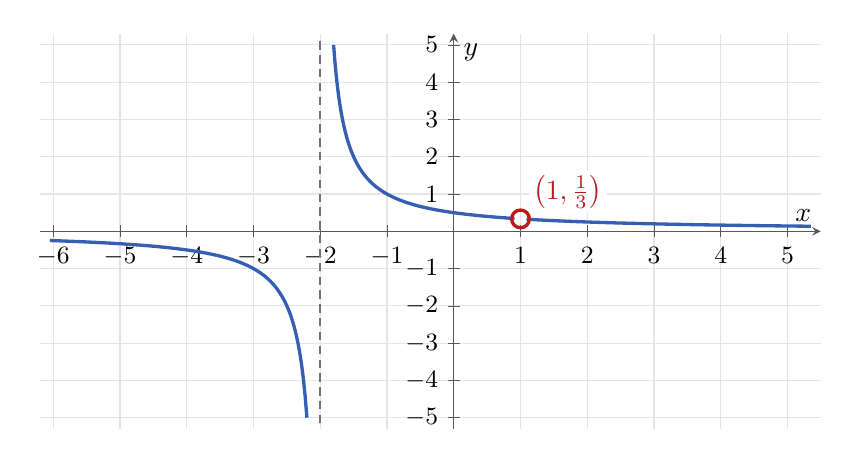
\begin{tikzpicture}
  \begin{axis}[
    width=11.5cm,
    height=6.6cm,
    axis lines=middle,
    xmin=-6.2,
    xmax=5.5,
    ymin=-5.3,
    ymax=5.3,
    xlabel={$x$},
    ylabel={$y$},
    xtick={-6,-5,-4,-3,-2,-1,1,2,3,4,5},
    ytick={-5,-4,-3,-2,-1,1,2,3,4,5},
    grid=major,
    grid style={black!10},
    axis line style={black!65},
    tick style={black!65},
    tick label style={font=\small},
    clip=false,
  ]
    \draw[guia, densely dashed, thick]
      (axis cs:-2,-5.15) -- (axis cs:-2,5.15);
    \addplot[corba, very thick, domain=-6.05:-2.2, samples=140]
      {1/(x+2)};
    \addplot[corba, very thick, domain=-1.8:0.91, samples=140]
      {1/(x+2)};
    \addplot[corba, very thick, domain=1.09:5.35, samples=140]
      {1/(x+2)};
    \addplot[
      only marks,
      mark=o,
      mark size=3.2pt,
      mark options={fill=white, draw=punt, line width=1.2pt}
    ] coordinates {(1,0.333333)};
    \node[anchor=south west, text=punt, fill=white, inner sep=1.5pt]
      at (axis cs:1.12,0.48) {$\left(1,\frac13\right)$};
  \end{axis}
\end{tikzpicture}
\end{document}
